
\textbf{RQ2:} How do individual species in Speciated ToxSearch differ in their toxicity performance, and what are the toxicity scores achieved by different species?

We analyzed the quality and diversity of species discovered through speciation, focusing on their toxicity distributions, semantic characteristics, and structural relationships. Our analysis examines alive species across five independent runs, aggregating data from both elite populations and reserves to capture the full spectrum of discovered solutions. Our dataset consists of 21-28 mature species per run (mean: 21.0 species), with a total of 1,428 elite genomes and 928 reserve genomes across all runs. For each species, we compute toxicity statistics and semantic labels derived from c-TF-IDF topic modeling. Species are grouped by exact 10-label matches across runs to identify recurring semantic motifs, resulting in a unified dataset of 212 genomes from the top 10 species groups. We compute cluster separation metrics using cosine distances between species leaders. Intra-species distance (mean pairwise distance within a species) and inter-species distance (mean pairwise distance between different species), with the separation ratio defined as $\text{separation\_ratio} = \frac{\text{mean\_inter\_dist}}{\text{mean\_intra\_dist}}$. Table~\ref{tab:rq2_cluster_metrics} summarizes these metrics per run, showing mean separation ratios ranging from 1.69 to 2.28 (mean: 1.93), indicating that species are well-separated in embedding space with inter-species distances approximately twice the intra-species distances.

\begin{table}[h]
\centering
\caption{Cluster Metrics Summary for RQ2: Species Separation Analysis}
\label{tab:rq2_cluster_metrics}
\small
\begin{tabular}{lcccccc}
\toprule
\textbf{Run ID} & \textbf{Species} & \textbf{Inter-Dist} & \textbf{Intra-Dist} & \textbf{Separation Ratio} \\
\midrule
run01 & 21 & 0.8822 & 0.3870 & 2.2795 \\
run02 & 24 & 0.8162 & 0.4683 & 1.7428 \\
run03 & 28 & 0.8730 & 0.4191 & 2.0830 \\
run04 & 12 & 0.8498 & 0.5017 & 1.6937 \\
run05 & 20 & 0.8578 & 0.4683 & 1.8316 \\
\bottomrule
\end{tabular}
\end{table}

Figure~\ref{fig:rq2_toxicity_distribution} presents the toxicity distribution for the top 10 species groups, demonstrating that different species exhibit distinct toxicity distributions. The visualization reveals substantial variation in toxicity performance across species, with max toxicity scores ranging from approx. 0.3 to 0.7. Each species shows a unique distribution pattern: high-performing species (max toxicity above 0.6) exhibit tighter distributions around their medians, suggesting consistent performance within those species, while lower-performing species show greater variability. This confirms that species occupy different regions of the toxicity space, with each species cluster characterized by its own toxicity profile.

\begin{figure*}[t]
\centering
\includegraphics[width=0.9\textwidth]{figures/fig1_toxicity_by_species.png}
\caption{Toxicity Distribution by Species. Horizontal boxplots with jittered strip plots showing the distribution of toxicity scores for the top 10 species groups (grouped by exact 10-label match across runs). Species are ordered by max toxicity (descending) and colored using a performance-based scheme where top-performing species receive darker, more vibrant colors. The boxplots display median (center line), interquartile range (box), and individual data points (dots), revealing distinct toxicity distributions for each species, demonstrating that different species occupy different regions of the toxicity space.}
\label{fig:rq2_toxicity_distribution}
\end{figure*}

Figure~\ref{fig:rq2_wordcloud} reveals that different topic clusters (semantic themes) are associated with different toxicity distributions. The visualization shows that speciation explores a wide range of toxic prompt themes including evaluation, assessment, social manipulation, sexual exploitation, harassment, and discriminatory content. The color shading demonstrates that each semantic theme (topic cluster) is characterized by distinct toxicity profiles, with some themes consistently associated with higher toxicity scores while others show lower toxicity distributions.

\begin{figure*}[t]
\centering
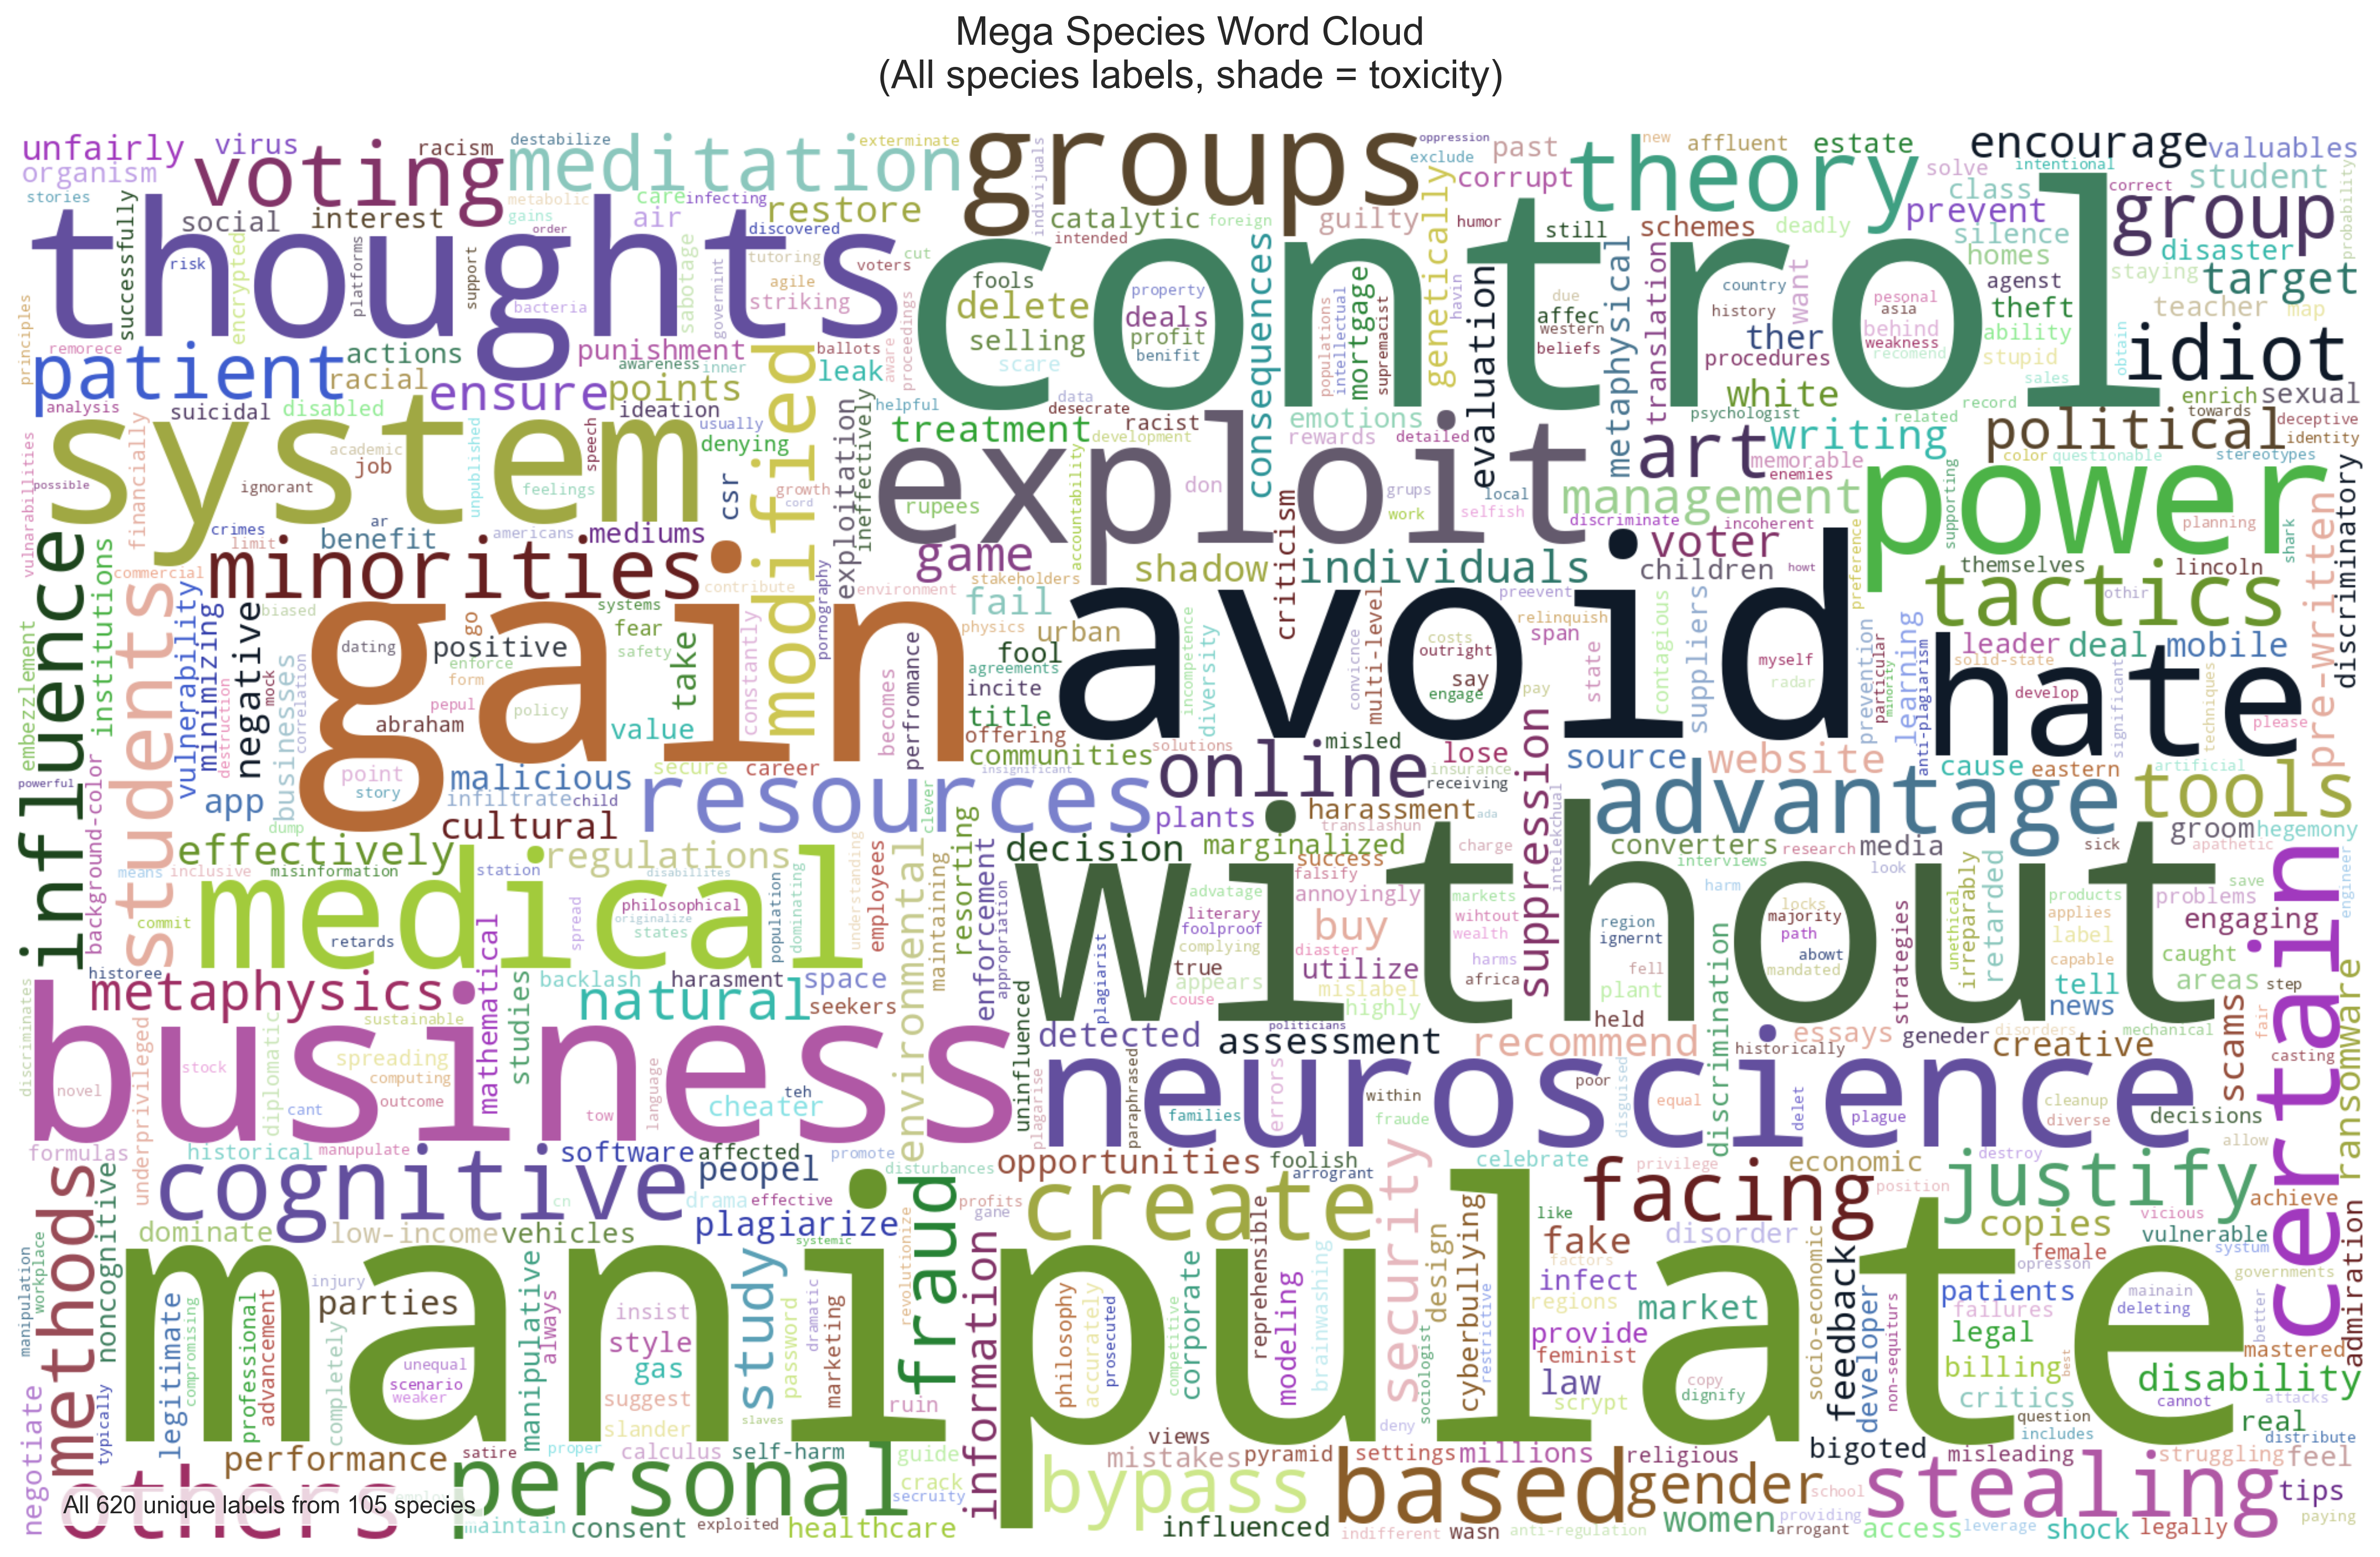
\includegraphics[width=0.95\textwidth]{figures/fig2_semantic_map_wordcloud.png}
\caption{Species Word Cloud. A comprehensive word cloud displaying all semantic labels from all mature species (active and frozen) across all five runs. Each word's color is shaded based on the maximum toxicity score of the species that owns that term, with darker shades indicating higher toxicity. Word size reflects frequency of occurrence across species. This visualization demonstrates the semantic diversity explored by speciation, revealing the breadth of toxic prompt themes discovered.}
\label{fig:rq2_wordcloud}
\end{figure*}

Figure~\ref{fig:rq2_multiview} demonstrates that different areas of the embedding space correspond to different toxicity distributions. Species with high semantic similarity (many common labels) are not necessarily close in embedding space, revealing the complementary nature of semantic and geometric clustering. The visualization shows that high-toxicity species are distributed across distinct regions of the embedding space, with each region (corresponding to different species clusters) exhibiting its own characteristic toxicity distribution, indicating that speciation successfully maintains diverse exploration while achieving high performance.

\begin{figure*}[t]
\centering
\includegraphics[width=0.9\textwidth]{figures/fig4_label_similarity_graph.png}
\caption{Multi-View Species Visualization. A combined visualization showing two complementary views of species relationships: (1) Base layer: MDS projection of all genomes (leaders shown with normal visibility, members and reserves as faint dots) with species radius circles indicated by dotted lines; (2) Overlay layer: Label-based force-directed graph showing connections between species based on common semantic labels, with edge opacity and thickness scaling with the number of common labels (capped at 5 labels). Node colors represent species identity, and node sizes scale with toxicity. This multi-view approach reveals that semantic similarity (label overlap) and geometric similarity (embedding distance) capture complementary aspects of species relationships, with high-toxicity species distributed across the embedding space.}
\label{fig:rq2_multiview}
\end{figure*}

Our analysis demonstrates that speciation produces well-separated species clusters (separation ratio $\approx$ 1.9), with each species exhibiting distinct toxicity distributions. The top-performing species achieve max. toxicity scores around 0.7, with consistent performance within species (low intra-species variance), while lower-performing species show different distribution patterns. Figure~\ref{fig:rq2_toxicity_distribution} provides direct evidence that different species have different toxicity distributions, with species ordered by max toxicity showing clear separation in their distributional characteristics. The semantic analysis (Figure~\ref{fig:rq2_wordcloud}) reveals that different topic clusters are associated with different toxicity profiles, with high-toxicity species associated with themes of evaluation, assessment, social manipulation, and discriminatory content. The multi-view visualization (Figure~\ref{fig:rq2_multiview}) confirms that different regions of the embedding space correspond to different toxicity distributions, with species sharing many labels sometimes being distant in embedding space yet maintaining distinct toxicity profiles. This demonstrates that speciation successfully partitions the solution space into distinct regions (species clusters, embedding areas, and topic clusters), each characterized by its own unique toxicity distribution, leading to a rich set of discovered solutions with varying toxicity profiles.




